\chapter{WebGL Rendering Library}
\label{chp:WebGL Rendering Library}

To be able to show dynamically generated images in a browser - in the sense of a picture rendered directly from a scene - there are different tools and APIs. However, as \textit{Awe.js} uses \textit{Three.js} as the underlying rendering library, only this library will be observed to create a better understanding on how \textit{Awe.js} works in the base and how it could possibly be adapted.

\section{Three.js and WebGL}

According to \cite{Profenza2010Three.jsOverflow}, "Three.js is a lightweight cross-browser JavaScript library/API used to create and display animated 3D computer graphics on a Web browser. Three.js scripts may be used in conjunction with the HTML5 canvas element, SVG or WebGL."

WebGL - standing for Web Graphics Library - is described by \cite{ComputerHope2017WebGL} as "a JavaScript API that allows compatible web browsers to render 2D and 3D graphics without the assistance of a plug-in. WebGL is written in a mix of JavaScript and shader code, executed by the GPU. . . . WebGL is based on OpenGL ES 2.0 and uses the HTML5 canvas element." 

Although \textit{Three.js} has a fallback for non WebGl-capable browsers, it is recommended for performance reasons - as the use of the GPU make rendering faster - to use a browser that supports WebGl. Whether a browser actually supports WebGL can be tested at \url{https://get.webgl.org/}.

In my opinion the big advantage of the \textit{Three.js} library is that it comes with a certain level of complexity and that it handles the rendering in a neat way without having to take care about the actual APIs used to get along with WebGL.

On their official web side \url{https://threejs.org/} the \textit{Three.js} team provides - besides the  documentation including also coding examples and the free access to download the library\footnote{The \textit{Three.js} library is also on GitHub at \url{https://github.com/mrdoob/Three.js/}} - examples of some projects realised with the use of \textit{Three.js} which equally serves  as a reference for what more can be done with this library.


\section{Base Code}

To start with \textit{Three.js} the library itself is needed. It could be linked in directly via \url{https://threejs.org/build/three.min.js}. For reproduction reasons of this project I downloaded the \textit{Three.js} ZIP-archive \footnote{ZIP-archive of \textit{Three.js} at \url{https://github.com/mrdoob/Three.js/archive/master.zip}} and put the library JavaScript file \textit{three.min.js} and all other needed files into the \textit{Applications/Chapter2/third-party/} folder. All files in that folder will remain as they are provided in the \textit{Three.js} ZIP-archive. The downloaded archive is in the \textit{Source/third-party} folder.

The HTML-file \mbox{\textit{baseCode.html}} was build accordingly to the \textit{Three.js} documentation\footnote{The  \textit{Three.js} documentation is available online at \url{https://threejs.org/docs/index.html}} of \textit{Creating a scene}\footnote{Online at \url{https://threejs.org/docs/\#manual/en/introduction/Creating-a-scene}} by \cite{Mr.doob2018Three.js/docs/manual:Creating-a-scene.html} and is directly locally executable in the browser.

The result is a green cube rotating on a black background like shown in figure \ref{fig:green cube}.

\begin{figure}[h]
    \centering
    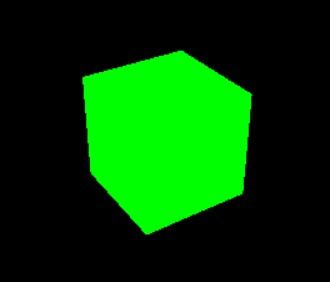
\includegraphics[height=4cm]{Document/Figures/chapter2/ScreenshotGreenCube.jpg}
    \caption[Screenshot of the green cube]{Screenshot of the green cube when running \textit{baseCode.html}}
    \label{fig:green cube}
\end{figure}



\section{Loading Objects}

To enhance the scene with more complex object beside the simple standard shapes, it needs a possibility to load an objects from a file. Using the example \textit{webgl loader obj} \footnote{Online at \url{https://threejs.org/examples/webgl_loader_obj.html}} by \cite{Mr.doob2012Three.js/examples:Webgl_loader_obj.html} as model I adapt \textit{baseCode.html} to create the new file  \textit{baseCodeExtendedObject.html}. 
There are the OBJ file \textit{male02.obj} and the \textit{OBJLoader.js} - that extends the \textit{Three.js} library and has to be linked in separately -  which are both provided in the \textit{Three.js} ZIP-archive and which I put into the \textit{third-party} folder. Despite that the example uses texture loading  only the loading of the object is added in this step to keep things clean and observable. Instead of a texture a standard wire frame material is used to give the objects a visible shape. The animation was commented out as it is not needed for this demonstration and render request - that was nested inside \textit{animate} - is moved outside and just called when an object has to be rendered. Scaling and positioning an object in \textit{Three.js} is intuitively by setting the x,y,z of the \textit{scale} and \textit{position} properties of an object. Running {baseCodeExtendedObject.html} shows a green wired cube and a figure of a man with the same material as the cube like in figure \ref{fig:cube and man}. 

\begin{figure}[h]
    \centering
    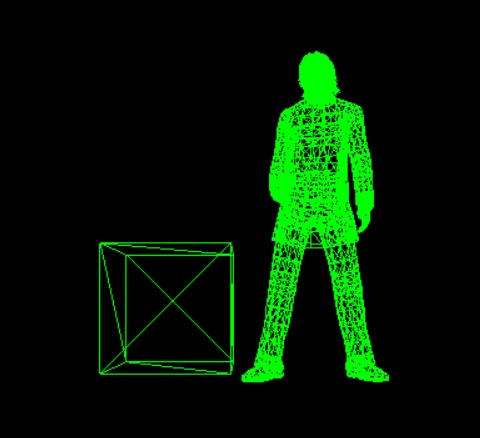
\includegraphics[height=4cm]{Document/Figures/chapter2/ScreenshotLoadedObject.jpg}
    \caption[Screenshot of the green wired cube and man]{Screenshot of the green wired cube and man when running \mbox{\textit{baseCodeExtendedObject.html}}}
    \label{fig:cube and man}
\end{figure}

This file can not be executed directly locally in the browser because of its use of a \textit{XMLHttpRequest} and the browsers' same origin policy security restrictions. This is pointed out in the guide \textit{How to run things locally}\footnote{Online at \url{https://threejs.org/docs/\#manual/en/introduction/How-to-run-things-locally}} by \cite{Anaranjo972018Three.js/docs/manual:How-to-run-things-locally.html}. They suggest to either change the security settings or to run the file on any kind of server such as a web server or the local host.

However this method is very nice - especially when the application will run on some sort of server -  I will avoid objects that has to be loaded that way to ease the use of the final application.

\section{Loading Textures}

Despite the cross origin problem for loading some object with \textit{Three.js}, the new implementation of the \textit{TextureLoader}\footnote{Online at url{https://threejs.org/docs/\#api/en/loaders/TextureLoader}} able to set the cross origin looked promising. However its implementation in \textit{baseCodeExtendedTexture.html} run into the same problems as the object loader. 

Trying to load the image into the DOM and uses it this way like \cite{2pha2015JavascriptOverflow} did in his answer does not work out when running {baseCodeExtendedTexture.html} locally.

Therefore the verdict for the texture loader is the same as for the object loader and I try to avoid loading textures. Nevertheless, if it is needed to load a texture and the use of either the local host or a web server is given  the \textit{TextureLoader} provides a nice one-liner to create a material with a loaded texture. Using the texture from the example {webgl loader obj} placed into the \textit{third-party} folder will show the cube with the applied texture as in figure \ref{fig:textured cube}.

\begin{figure}[h]
    \centering
    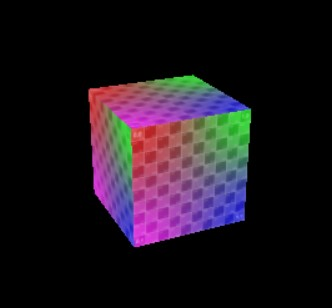
\includegraphics[height=4cm]{Document/Figures/chapter2/ScreenshotTexturedCube.jpg}
    \caption[Screenshot of the cube applied the texture on it]{Screenshot of the cube applied the texture on it when  running \mbox{\textit{baseCodeExtendedObject.html}}}
    \label{fig:textured cube}
\end{figure}

\section{Materials and Lights}

Without texture, the cube would look like in the \textit{baseCode.html} example where the edges are not really visible. As shown in the tutorial by \cite{Lewis2012AerotwistThree.js} this can be changed easily by creating a material - \textit{THREE.MeshLambertMaterial} - that interacts with light and match it to the cube. However without a light it is not visible at all. Therefore a light - \textit{THREE.PointLight} - is added. Those commands are contain in \textit{Three.js} and has just to be applied to the scene. Running \mbox{\textit{baseCodeExtendedMaterialAndLight.html}} will show a red cube with visible edges due to the lighting a shown in figure \ref{fig:red cube}.

\begin{figure}[h]
    \centering
    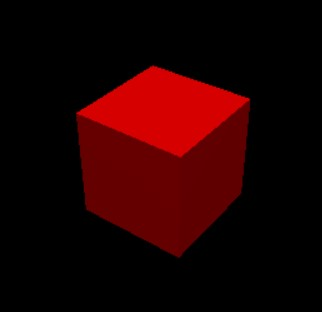
\includegraphics[height=4cm]{Document/Figures/chapter2/ScreenshotRedCubeWithLight.jpg}
    \caption[Screenshot of the red cube with light]{Screenshot of the red cube with light when  running \mbox{\textit{baseCodeExtendedMaterialAndLight.html}}}
    \label{fig:red cube}
\end{figure}

\section{Manipulating Objects}
\label{sec:Manipulating Objects}

In the previous steps it showed already, that \textit{Three.js}provides a neat way to apply geometric operations on the object. Object can be translated by accessing the \textit{position} property, rotated and scaled in any of the three axis x, y and z. Like that a object can be animated pragmatically by changing those values inside the code in the animation cycle. To gain control over this changing and manipulation of values, the user should be able to interact with the code from outside during the run time. 

Observing the tw\textit{Three.js} examples \url{https://threejs.org/examples/webgl_animation_skinning_blending.html} and \url{https://threejs.org/examples/webgl_animation_skinning_morph.html} I found that they use another library for adding weight slider and control panels which could come in handy for later. This library is called \textit{dat.GUI} and can either be found on its own GitHub repository at \url{https://github.com/dataarts/dat.gui} or again in the big collection of the \textit{Three.js} ZIP-archive. The library file \textit{dat.gui.min.js} is also place in the \textit{third-party} folder.

Inspired by the two examples I extended the base code to a new version \textit{baseCodeExtendedManipulation.html}. For further understanding of \textit{dat.GUI} there is a workshop at \url{https://workshop.chromeexperiments.com/examples/gui/}. By instantiating the GUI, it is placed right away on the screen and is ready to go. Different types of customizable variable are added with ease. Running {baseCodeExtendedManipulation.html} - that is directly locally executable - shows the cube influenced by some manual changed parameters over the \textit{dat.GUI} panel represented in figure \ref{fig:cube and panel}.

\begin{figure}[h]
    \centering
    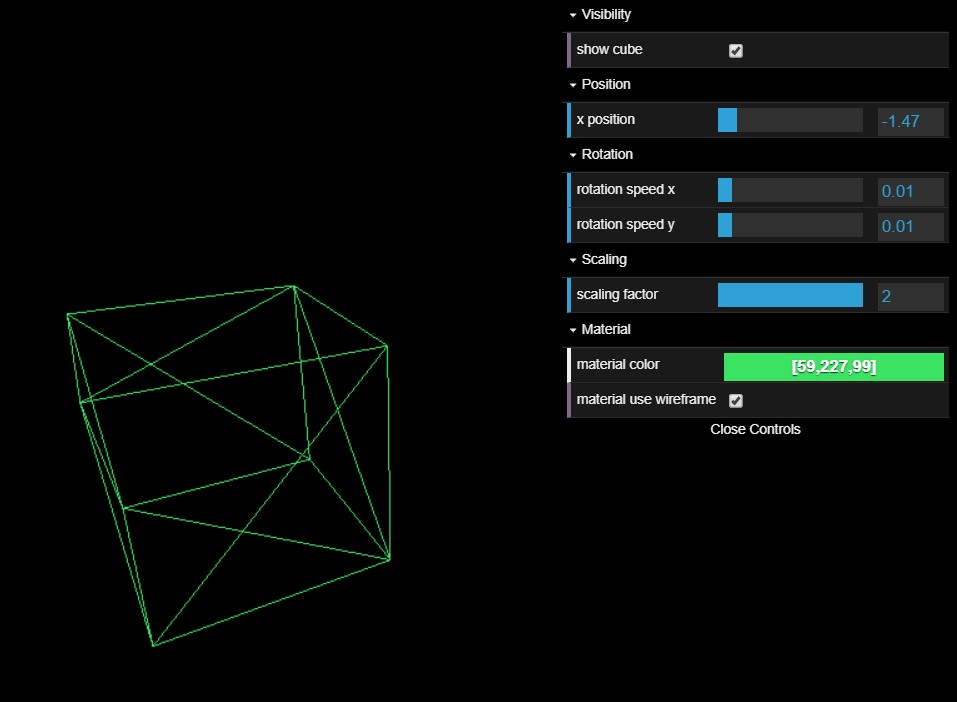
\includegraphics[height=5cm]{Document/Figures/chapter2/ScreenshotManipulation.jpg}
    \caption[Screenshot of the \textit{dat.GUI} panel and the cube]{Screenshot of the \textit{dat.GUI} panel and the cube with the parameters applied on it when running \mbox{\textit{baseCodeExtendedObject.html}}}.
    \label{fig:cube and panel}
\end{figure}

\section{Evaluation}

\textit{Three.js} is a grate library that has a lot of great functionalities build in and is even expandable with more features.
keep in mind

could use some lights and more complex materials to apply on the scene, however the above mentioned steps should be enough to keep the balance like so that the creation of the scenes stays simply but has already some aesthetics.

It is possible to render simple or complex objects and connect them with a texture. It is also possible to manipulate objects and their animation.

You can create a scene and animate things. For this bit of code I adapted the structure of the given example for the reason of overview and extensibility. You do not have to be aware of the rendering and the actual handling of the object, which is done in the Three.js library.

Keep in mind, that device has to calculate -> keep it simple to calculate (for example: back to box with simple material)

also: light and controls (user interaction) will come later.
So it is more to understand the concept and to see, whether the basics work
